\documentclass{article}
\usepackage{frExamplee, times}
%%\usepackage{graphicx}
%%\usepackage{apalike}
\usepackage{setspace}
\input{./latexGoodPractices/preamble}
\addbibresource{./references.bib}

% Add subfigure
\usepackage{subcaption}

% Add figure with caption at the side
\usepackage{sidecap}

% For dates and time
\usepackage{datetime2}
\DTMnewtimestyle{custom}{
	\renewcommand{\DTMdisplaytime}[3]{
		\DTMtexorpdfstring{\DTMtwodigits{##1}:\DTMtwodigits{##2}}
	}
}
\DTMsettimestyle{custom}

%For tikz figure
\usepackage{tikz}
\usepackage{pgfplots}
\usepackage{csvsimple}
\usetikzlibrary{shapes}

% For checkmarks
\usepackage{pifont}% http://ctan.org/pkg/pifont
\newcommand{\cmark}{\ding{51}}%
\newcommand{\xmark}{\ding{55}}%


% Text commands
\newcommand{\laverdiere}{Laverdi\`{e}re} % Laverdière
\newcommand{\quebec}{Qu\'{e}bec} % Québec
\newcommand{\foretmo}{For\^{e}t Montmorency} % Québec

% Useful math commands
\newcommand{\mapf}{\mathcal{G}} % map reference frame
\newcommand{\odomf}{\mathcal{O}} % odom reference frame
\newcommand{\robotf}{\mathcal{R}} % robot reference frame
\newcommand{\lidarf}{\mathcal{L}} % lidar reference frame
\newcommand{\pathf}{\mathcal{S}} % path Frenet-Serret frame
\newcommand{\skreadpc}{\check{\mathcal{P}}} % Skewed reading point cloud
\newcommand{\readpc}{\mathcal{P}} % reading point cloud
\newcommand{\refpc}{\mathcal{Q}} % reference point cloud
\newcommand{\match}{\mathcal{M}} % set of point matches
\newcommand{\weight}{\mathcal{W}} % set of point weights
\newcommand{\transform}[2]{$_{#1}^{#2}\bm{T}$} % Transform from #1 frame to #2 frame

% argmin and argmax
\DeclareMathOperator*{\argmin}{arg\,min}

%JL: is there a specific reason for this notation? I find the notation _^{R1}T_{R2} somewhat better, but it might be personal!


\title{Lidar-based teach-and-repeat in subarctic conditions}

\author{
Dominic Baril\thanks{ Use footnote for providing further information
	about author (webpage, alternative address). Acknowledgments to
	funding agencies should go in the \textbf{Acknowledgments} section
	at the end of the paper.} \\
Norlab, Universit\'{e} Laval\\
Qu\'{e}bec, QC, Canada G1V 0A6 \\
\texttt{dominic.baril@norlab.ulaval.ca} \\
\And
Simon-Pierre Desch\^{e}nes \\
Norlab, Universit\'{e} Laval\\
Qu\'{e}bec, QC, Canada G1V 0A6 \\
\And
Olivier Gamache \\
Norlab, Universit\'{e} Laval\\
Qu\'{e}bec, QC, Canada G1V 0A6 \\
\And
Maxime Vaidis \\
Norlab, Universit\'{e} Laval\\
Qu\'{e}bec, QC, Canada G1V 0A6 \\
\And
Damien Larocque \\
Norlab, Universit\'{e} Laval\\
Qu\'{e}bec, QC, Canada G1V 0A6 \\
\And
Johann Laconte \\
Norlab, Universit\'{e} Laval\\
Qu\'{e}bec, QC, Canada G1V 0A6 \\
\And
Vladim\'{i}r Kubelka \\
Norlab, Universit\'{e} Laval\\
Qu\'{e}bec, QC, Canada G1V 0A6 \\
\And
Philippe Gigu\'{e}re \\
Norlab, Universit\'{e} Laval\\
Qu\'{e}bec, QC, Canada G1V 0A6 \\
\And
Fran\c{c}ois Pomerleau \\
Norlab, Universit\'{e} Laval\\
Qu\'{e}bec, QC, Canada G1V 0A6 \\
\texttt{francois.pomerleau@norlab.ulaval.ca} \\
}

% The \author macro works with any number of authors. There are two commands
% used to separate the names and addresses of multiple authors: \And and \AND.
%
% Using \And between authors leaves it to \LaTeX{} to determine where to break
% the lines. Using \AND forces a linebreak at that point. So, if \LaTeX{}
% puts 3 of 4 authors names on the first line, and the last on the second
% line, try using \AND instead of \And before the third author name.

% Acronym definitions
\acrodef{SNOW}{Self-driving Navigation Optimized for Winter}
\acrodef{SSMR}{Skid-steering mobile robot}
\acrodef{UGV}{unmanned ground vehicle}
\acrodef{GPR}{ground penetrating radar}
\acrodef{IMU}{inertial measurement unit}
\acrodef{GPS}{Global Positioning System}
\acrodef{RTK}{Real-time Kinematics}
\acrodef{GNSS}{Global Navigation Satellite System}
\acrodef{ICP}{iterative closest point}
\acrodef{SLAM}{Simultaneous Localization and Mapping}
\acrodef{DoF}{degree of freedom}
\acrodef{ICR}{instantaneous centre of rotation}
\acrodef{ROC}{radius of curvature}
\acrodef{COM}{center of mass}
\acrodef{ROS}{Robot Operating System}
\acrodef{MPC}{Model Predictive Control}
\acrodef{VTR}[VT\&R]{Visual Teach and Repeat}
\acrodef{LTR}[LT\&R]{Lidar Teach and Repeat}
\acrodef{EBN}{Experience-based navigation}
\acrodef{MEL}{Multi-experience Localization}
\acrodef{CNN}{Convolutional Neural Network}
\acrodef{GeRoNa}{Generic Robot Navigation}
\acrodef{ORTHEXP}{Orthogonal-Exponential}
\acrodef{DD-ORTHEXP}{Differential-Drive-ORTHEXP}
\acrodef{POI}{Points of Interest}

\begin{document}

\maketitle

\begin{abstract}
\lightlipsum[1]
\end{abstract}

\section{Introduction}
\label{sec:intro}

\lightlipsum[1]
\cite{Pomerleau2014}

\begin{figure} [h]
	\centering
	\includegraphics[height=2.0in]{example-image}
	\caption{Warthog driving / Aerial shot of the different paths}
	\label{fig:front_fig}
\end{figure}

\lightlipsum[1]
\lightlipsum[1]
\lightlipsum[1]
\section{Related work}
\label{sec:rel_work}

\subsection{Robotic deployments in snow}
\label{sec:snow_robots}

To our knowledge, few robots have been deployed in harsh winter environments. 
Dante II is a \SI{900}{kg} tethered legged robot, which conducted a 5-day, \SI{165}{m} descent into the Mount Spurr Volcano, in Alaska~\citep{Bares1999}.
During this deployment, Dante II reached speeds upwards to \SI{0.011}{m/s} during the descent.
A two-axis lidar was used to create a local elevation map around the robot in order to conduct autonomous navigation.

Nomad is a gasoline-powered \SI{725}{kg} \ac{UGV}, was deployed at Elephant Moraine, Antarctica for a duration of 4 weeks~\citep{Apostolopoulos2000}. 
The robot reached speeds upwards of \SI{0.5}{m/s} while using differential-\ac{GPS} as the primary method of localization.
The platform also used stereo cameras and a lidar sensor for obstacle detection, although stereo vision was found to be ineffective  on blue ice and snow in Antarctica due to extreme lack of texture~\citep{Moorehead1999}.
Roll/pitch/yaw sensors were also added to the robot to make it cognizant to hazardous terrain.
Nomad achieved its initial goal to identify meteorites autonomously in Antarctica at a search rate of ~  \SI{160}{m^2/h}.

MARVIN I and MARVIN II are two diesel-powered \acp{SSMR} weighing \SI{720}{kg} were deployed in Greenland~\citep{Stansbury2004} and Antarctica~\citep{Gifford2009} respectively. 
The goal of these robots was to increase survey safety in remote polar regions and large sensor payloads led to the selection of large vehicles.
Both vehicles used \ac{RTK} \ac{GPS} as primary method, achieving a centimeter-level accuracy.
They also used a lidar sensor for obstacle detection and a a gyroscope and inclinometer were used to provide the robot's pitch and roll angles.
Skid-steer turns often caused MARVIN I to get immobilized in snow and its transmission eventually broke down during operation.
MARVIN II thus incorporated design improvements to the hydro-static drive and track systems to increase its durability.


Sno-mote Mk1 and Mk2 are dual-drive 1:10 scale snowmobiles equipped with a single camera and \ac{GPS} antenna were deployed on Alaskan glaciers and Wapekoneta, Ohio~\citep{Williams2009}.
These robots were used to conduct manually-driven traverses of about \SI{100}{m} at a speed of ~\SI{1}{m/s}.
The data gathered with the Sno-motes was then used to improve visual \ac{SLAM} feature extraction methods in snow. 
Despite improving feature detection methods on snow, it was shown that snow is still feature-sparse~\citep{Williams2009}.
Through this work, improvements were also done on slope estimation~\citep{Williams2010} and horizon line estimation~\citep{Williams2011}.

Yeti is a battery-powered \SI{81}{kg} \ac{UGV} in Antarctica and Greenland~\citep{Lever2013}. 
Yeti was used to conduct \ac{GPR} surveys in order to detect subsurface crevasses or other voids to increase vehicle travel safety in remote polar environments.
Since polar terrain is largely obstacle-free and the effort required to provide reliable obstacle detection on low-contrast snowfields is considerable, Yeti drove "blind", relying only on \ac{GPS} waypoint following.
During surveys, Yeti reached a top speed of \SI{2.2}{m/s} and managed to acquire data on hundreds of crevasse encounters and even locate a previously undetected buried building in the South Pole.

A Clearpath Robotics Grizzly, a battery- and gasoline-powered \ac{SSMR} was deployed during winter on the University of Toronto Institute for Aerospace Studies (UTIAS) campus, in Ontario, Canada~\citep{Paton2017}.
Only stereo cameras were used through a visual \ac{SLAM} algorithm to localize the robot during autonomous teach-and-repeat runs. 
Path tracking was accomplished using a \ac{MPC} algorithm.
A 250 m path was successfully repeated on an light snow cover 3 hours after it was first manually driven. 
However, deep snow path-following provided unsatisfactory results due to features almost only being observed on the horizon, leading to inaccurate pose estimates, which caused issues for the path tracker.
Furthermore, vehicle tracks that constantly change when driven over lead to an increased pose estimation error.

A full-scale battery-powered Toyota Prius was deployed during winter on roads in Massachusetts, USA~\citep{Ort2020}.
Localization was accomplished using a custom-designed localizing \ac{GPR}. 
A prior mapping must be conducted during which the driven is driven by a human operator and the vehicle's sensor data is recorded, the saved map can then allow the vehicle to localize within this area.
The \ac{GPR} location information is then probabilistically fused with wheel odometry and \ac{IMU} measurements to provide accurate vehicle localization.
Path tracking is accomplished through the use of a Pure Pursuit controller, specifically designed for Ackermann steered autonomous vehicles.
The system showed similar performance in localization accuracy (\SI{0.34}{m} to \SI{0.39}{m}) and cross-track error (\SI{0.26}{m} to \SI{0.29}{m}) between clear weather and snow-covered road.
The localizing \ac{GPR} sensor's measurement range depends on the width of the array, meaning the system cannot be easily miniaturized, which means it was mounted on the rear of the vehicle, at \SI{32}{cm} above the ground.
This sensor size and mounting requirement could lead to decreased performance in deep snow or in off-road environments. 

\subsection{Relative navigation}
\label{rel_nav}



% UofT TnR and other relevant
\lightlipsum[1]
\lightlipsum[1]
\section{System description}
\label{sec:sys}

This section will present a detailed description of our \ac{LTR} system. 
Our system was designed to work by using 3D lidar scans as a primary mean of localization, also using \ac{IMU} and wheel odometry as input. 
The main components of the framework are shown in~\autoref{fig:ltr_flow}.
As the \ac{ICP} algorithm is the foundation of this algorithm, our implementation of the \ac{ICP} algorithm is detailed first. 
Next, the teach phase is described, explaining how the reference trajectory and map are logged.
Subsequently, the repeat phase is described, when the robot localizes within the map a simple controller allows computing commands that allow to repeat the reference trajectory.
Finally, the hardware used to deploy the \ac{LTR} system, including the \ac{UGV}, sensing and computing hardware is described.

\begin{figure} [htpb]
	\centering
	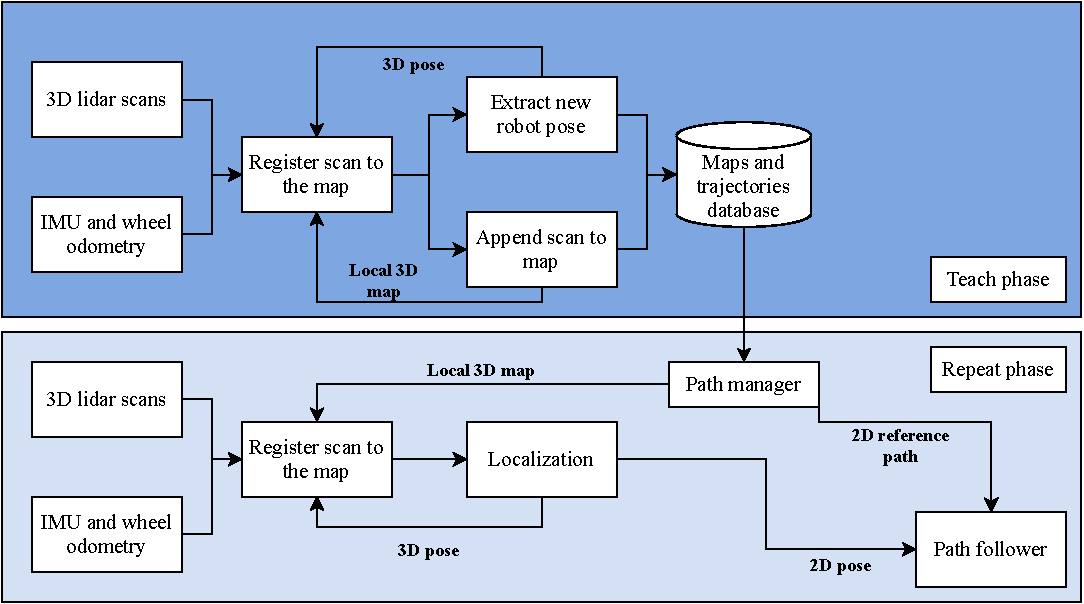
\includegraphics[height=3.2in]{figs/LTR_flowchart.pdf}
	\caption{Flowchart for LTR}
	\label{fig:ltr_flow}
\end{figure}

Various coordinate frames need to be defined for the \ac{LTR} framework to work, all of which are illustrated in~\autoref{fig:ltr_frames}.
First, a map frame $\mapf$ is defined representing the world in which the robot is navigating.
Second, a robot frame $\robotf$ is defined with its origin at the base of the robot chassis and the $x$-axis parallel to the longitudinal direction and the $y$-axis parallel to the lateral direction of the vehicle.
%The rigid transform \transform{\robotf}{\odomf} is updated at the rate of the \ac{IMU} and wheel odometry and used as a prior for the \ac{ICP} algorithm.
Thirdly, a lidar frame $\lidarf$ is defined at the origin of the lidar sensor. 
The rigid transform from the robot frame to the lidar frame \transform{\robotf}{\lidarf} is assumed to be constant and found through system calibration.
Reading point clouds $\readpc$ are originally observed in the lidar frame $\lidarf$ and reference point clouds are expressed in the map frame $\mapf$.
The transform between $\robotf$ and $\mapf$ \transform{\robotf}{\mapf} is updated via the \ac{ICP} algorithm and is used as odometry for the robot.
Lastly, for path following algorithm, a Frenet-Serret frame $\pathf$ is defined directly on the path.

%% TODO : Replace with our version of the figure
\begin{figure} [htpb]
	\centering
	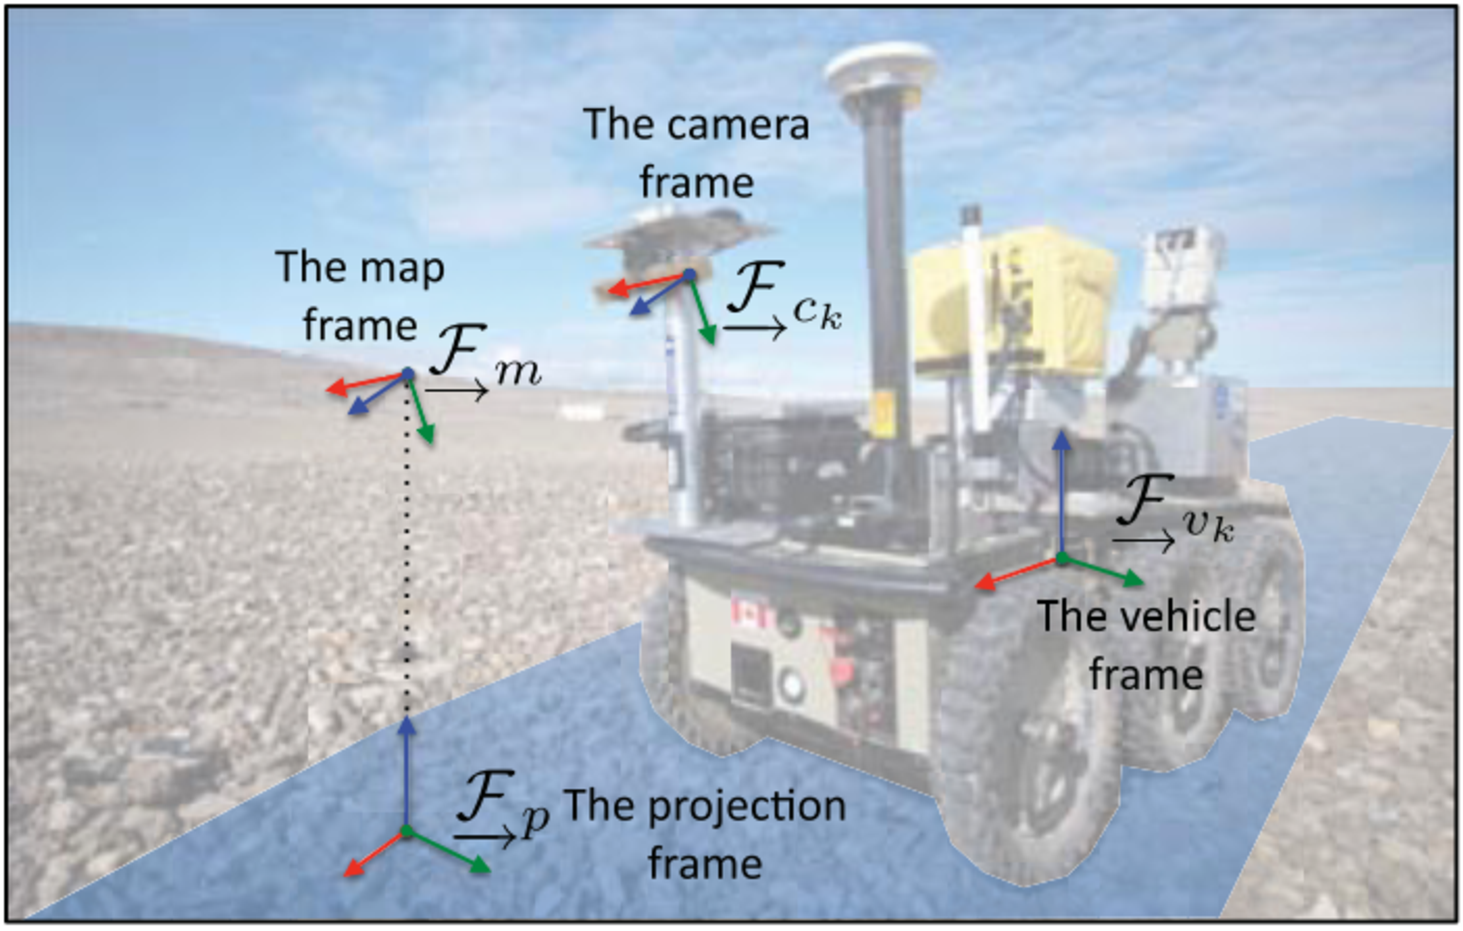
\includegraphics[height=2.0in]{figs/warthog_frames.pdf}
	\caption{Coordinate frames used for \ac{LTR}}
	\label{fig:ltr_frames}
\end{figure}

\subsection{Iterative closest point}
\label{ICP}

Incoming lidar scans, or reading point clouds $\readpc$ registered to a reference map, or reference point cloud $\refpc$ using the \ac{ICP} algorithm in order to localize the robot and build a map of the environment during the teach phase.
Pioneered by~\citet{Besl1992} and~\citet{Chen1991}, this algorithm iteratively matches points between two point clouds and looks for a rigid transform minimizing the distance between each matched points.
The first data processing step in our implementation is to randomly subsample $\readpc$ in order to decrease computation time.
In our implementation, we know that $\readpc$ is observed in the lidar frame $\lidarf$ and that $\refpc$ is defined in the map frame $\mapf$. 
Thus, the \ac{ICP} algorithm estimates the transform $_{\lidarf}^{\mapf}\bm{T}$ by minimizing an error function $\text{error}(\readpc, \refpc)$:

\begin{equation}
	_{\lidarf}^{\mapf}\bm{\hat{T}} = \argmin_{\bm T} (\text{error} \left(\readpc, \refpc, _{\lidarf}^{\mapf}\bm{\check{T}} \right))
\end{equation}

where $_{\lidarf}^{\mapf}\bm{\check{T}}$ is the prior transformation, estimated via the \ac{IMU} and wheel odometry.
In order to compute the error function, we associate points between $\readpc$ and $\refpc$.
This association is the done by finding the closest points in $\refpc$ for each point in $\readpc$, thus multiple points of $\refpc$ can be associated to each point of $\readpc$.
In order to accelerate this step, nearest neighbour search is done via the use of a kd-tree, as proposed by~\citet{Elseberg2012}.
In addition, binary weights are added to each point match in order to remove the outlier matches from the error function.
Formally, let $\match = \text{match}(\readpc, \refpc) = \{(\bm p, \bm q) : \bm p \in \readpc, \bm q \in \refpc \}$ be the set of matches between $\readpc$ and $\refpc$ and $\weight = \text{outlier}(\readpc, \refpc) = \{w(\bm p, \bm q) : \forall(\bm p, \bm q) \in \match\}$ be the weights associated to these matches.
Our system uses point-to-plane error, which can be computed as follows

\begin{equation}
	\text{error}(\readpc, \refpc) = \sum_{k=1}^{K} w(\bm p_k, \bm q_k) \lVert (\bm p_k - \bm q_k) \cdot \bm n_k \rVert_2
\end{equation}

where $K$ is the number of matches in $\match$ and $\lVert \cdot \rVert_2$ is the L2 norm. 
$\bm n_k$ is the normal vector around the 3D point $\bm q_k$ in $\refpc$, which needs to be computed prior to the \ac{ICP} algorithm.
This error can be iteratively minimized by recomputing $\match$ and $\weight$ at each iteration.
For more details, please refer to~\citep{Pomerleau2015}.
Once the optimal transform is found, $\readpc$ can be registered to $\refpc$ by applying it to every point of $\readpc$. 
The resulting points can then be appended to $\refpc$ and the resulting transform \transform{\lidarf}{\mapf} can be used to express the 3D robot pose in $\mapf$ by chaining \transform{\lidarf}{\mapf} \transform{\robotf}{\lidarf} since the latter is known through calibration.
Post filters are then computed on $\refpc$. 
The first consisting of computing the surface normals for all points in order to allow point-to-plane minimization.
The second one is used to filter out dynamic points in the map, following what was proposed by~\citet{Pomerleau2014}.
An overview of the \ac{ICP} pipeline is shown in~\autoref{fig:icp_pipeline}.
Our implementation is strongly based on the \texttt{libpointmatcher}\footnote{\url{https://github.com/ethz-asl/libpointmatcher}}~\citep{Pomerleau2013}.
The parameters that were used on our system are detailed in~\autoref{tab:icp_params}.

%% Need to write on point cloud preprocessing, matching, minimization (point-to-plane) and post-processing (might be added to mapping).

%% TODO : Re-do this figure to suit our needs for the paper
\begin{figure} [htpb]
	\centering
	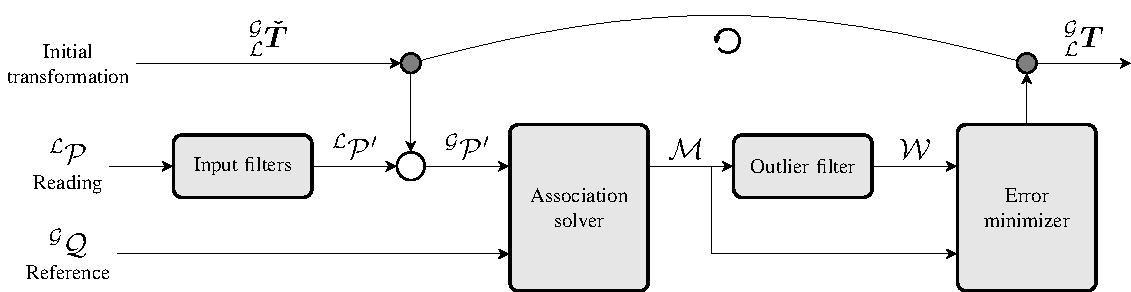
\includegraphics[width=\linewidth]{figs/icp_pipeline/icp_pipeline.pdf}
	\caption{ICP pipeline}
	\label{fig:icp_pipeline}
\end{figure}


\begin{table}[htpb]
	\caption{\ac{ICP} parameters} \label{tab:icp_params}
	\begin{center}
		\begin{tabular}{c c c c}
			\hline
			% after \\: \hline or \cline{col1-col2} \cline{col3-col4} ...
			ICP block & Function & Parameters & \\
			\hline
			General & & sensor\_max\_range = 80 \\			 
			& & min\_dist\_new\_point = 0.1 \\
			\hline
			Input filters & BoundingBoxDataPointsFilter & xMin: -1.5 & xMax: 0.5\\
			 & & yMin: -1 & yMax: 1  \\
			 & & zMin: -1 & zMax: 0.5 \\
			 & & removeInside: 1 \\
			 & BoundingBoxDataPointsFilter & xMin: -10 & xMax: -1.5\\
			 & & yMin: -2.5 & yMax: 2.5  \\
			& & zMin: -1 & zMax: 1 \\
			& & removeInside: 1 \\
			 & RandomSamplingDataPointsFilter & prob: 0.7 & \\
			\hline
			Matcher & KDTreeMatcher & knn: 7 & maxDist: 2.0 \\
			 & & epsilon: 1 \\
			\hline
			Outlier filter & TrimmedDistOutlierFilter & ratio: 0.7 & \\
			\hline
			Cost function & PointToPlaneErrorMinimizer & force4DOF: 1 & \\
			\hline
			Transformation & DifferentialTransformationChecker & minDiffRotErr: 0.001 & minDiffTransErr: 0.01 \\
			checkers & & smoothLength: 2 \\
			 & CounterTransformationChecker & maxIterationCount: 40 \\
			\hline
			Post filters & SurfaceNormalDataPointsFilter & knn: 15 \\
			 & CutAtDescriptorThreshold & descName: probabilityDynamic & useLargerThan: 1 \\
			 & & threshold: 0.8 \\
		\end{tabular}
	\end{center}
\end{table}

\subsubsection{\ac{IMU} and wheel odometry and point cloud de-skewing}
\label{sec:imu_wheel_odom}
%% Move before ICP
%% Skewed PC is inverse hat

As specified above, the \ac{ICP} algorithm requires high-frequency odometry to produce a prior estimate $_{\lidarf}^{\mapf}\bm{\check{T}}$.
This estimate is produced by estimating the robot displacement between lidar scans. 
Robot orientation is estimated using the Madwick filter\footnote{\url{https://github.com/bjohnsonfl/Madgwick_Filter}}~\citep{Madgwick2011} based on gyroscope and accelerometer measurements.
Linear displacement is estimated through vehicle body velocity commands.
Each command is propagated with the robot orientation between scans, yielding $_{\lidarf}^{\mapf}\bm{\check{T}}$ at a frequency of \SI{100}{Hz}.
In addition, it should be noted that lidar sensors typically make the assumption that the lidar frame $\lidarf$ is static during each scan, which is incorrect when the lidar sensors is subject to motion, yielding a skewed reading point cloud $\skreadpc$.
Hence, a point cloud de-skewing approach was added to our system.
First proposed by~\citet{Bosse2009}, such algorithms use the the high-frequency odometry to correct the location of each point before registration.
Following the same idea, our high-frequency odometry is used to estimate the de-skewed point cloud $\readpc$, which is the one that is used in the \ac{ICP} algorithm.


\subsection{Teach phase}
\label{sec:teach_phase}

During the teach phase, the robot is driven along a specific path by a human operator, while all sensors are used to collect data.
The \ac{ICP} algorithm is used to solve the \ac{SLAM} problem, hence incoming reading point clouds $\readpc$ are registered to the reference point cloud $\refpc$ and then appended to the reference, effectively building a map.
The other output of the \ac{ICP} algorithm, the transform that allows to register the reading point cloud to the reference point cloud \transform{\lidarf}{\mapf} represents the pose of the robot $\bm x$.
By logging all robot poses, we build a reference trajectory


\begin{figure} [htpb]
	\centering
	\includegraphics[height=2.0in]{example-image}
	\caption{Teach phase pipeline}
	\label{fig:teach_pipeline}
\end{figure}

\subsubsection{Tiled mapping for large scale}
\label{sec:tiled_map}
\lightlipsum[1]

\begin{figure} [htpb]
	\centering
	\includegraphics[height=2.0in]{example-image}
	\caption{Figure explaining Simon-Pierre's tiled mapping framework}
	\label{fig:tiled_map}
\end{figure}

\subsection{Repeat phase}
\label{sec:repeat_phase}

During the teach phase, the path map is loaded and used directly as the reference point cloud $\refpc$.
During this phase, the previously built maps are used to localize the robot while it follows the reference path.
Our system allows to repeat paths in both directions, going forwards or backwards. 
No obstacle detection feature was implemented on the system.
The repeat pipeline is shown in~\autoref{fig:repeat_pipeline}.

\begin{figure} [htpb]
	\centering
	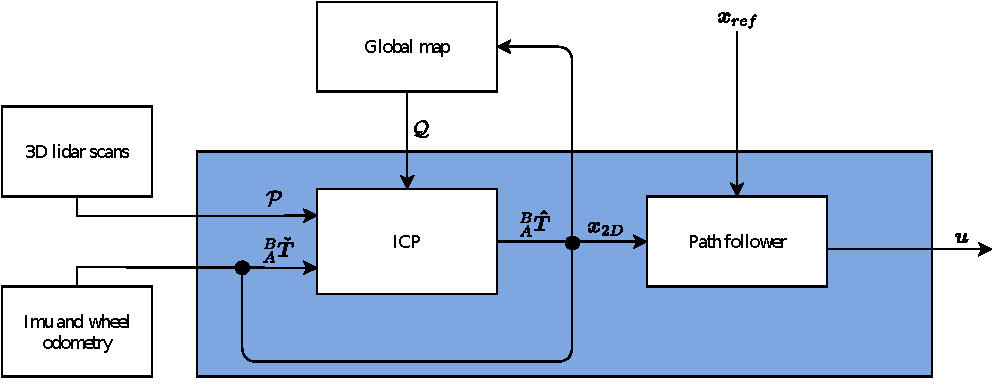
\includegraphics[height=2.0in]{figs/repeat_pipeline.pdf}
	\caption{Repeat phase pipeline}
	\label{fig:repeat_pipeline}
\end{figure}

\subsubsection{Repeat localization}
\label{sec:rep_loc}

\lightlipsum[1]

\subsubsection{Path following}
\label{sec:orthexp}

%% Review Frenet-Serret frame formulation from Huskic 2019

Once the robot is localized within the environment and the reference trajectory is defined, this information is used as input to a simple path following controller in order to complete the repeat pipeline.
The output of the path-following algorithm is the commanded longitudinal and angular velocities, defined in the vector $\bm u = [v_x, \omega]$.
For our implementation, we selected a simple \ac{ORTHEXP} controller. 
Originally proposed by~\citet{Mojaev2004} for differential-drive mobile robots, this controller allows path tracking with a feedback loop on robot localization.
This controller was later adapted for omnidirectional mobile robots by~\citet{Li2007} and for dribbling control for soccer robots.
More recently,~\citet{Huskic2017} improved the algorithm's path following performance through heuristic linear velocity control.
To implement this controller, we used the open-source \ac{GeRoNa}\footnote{\url{https://github.com/cogsys-tuebingen/gerona}} library, created by~\citet{Huskic2019}.

%Knowing the robot's 2D pose $\bm x_{\text{2D}}$ and reference trajectory $\bm x_{\text{ref}}$, it is possible to compute the orthogonal projection $\bm P$ of the robot on the reference path.
A Frenet-Serret frame $\pathf$ is defined within the map frame with its origin corresponding to the orthogonal projection of the robot on the reference pat.
For Frenet-Serret frame, abscissa $\bm x_t$ and ordinate $\bm x_n$ are unit tangent and unit normal vectors respectively. 
The orthogonal distance from the origin of the robot frame $\robotf$ and the Frenet-Serret frame $\pathf$ along the $\bm x_n$ axis is denoted with $x_n$ and the tangential distance with $x_t$.
The tangential angle of the Frenet-Serret frame $\pathf$ with respect to the map frame $\mapf$ is defined as $\theta_t$.
The angle of robot frame $\robotf$'s $\bm x$ axis with respect to the map frame $\mapf$ is defined $\theta_r$. %JL robot frame R's -> hard to read
If we denote $x_{n_o}$ as the distance between the origin of the robot frame $\robotf$ and the origin of the path frame $\pathf$, it is possible to define the following exponential law as
\begin{equation}
\label{eq:exp_law}
	x_n = x_{n_o} e^{-k x_t},
\end{equation}
where $k$ is a positive constant that allows to regulate the convergence speed of the robot to the path.
Next, the exponential function's tangent angle with the map frame $\phi_e$ can be computed as follows:
\begin{equation}
\label{eq:exp_angle}
\phi_e = \arctan(-k x_n).
\end{equation}

The angular velocity command can then be computed as %JL: remove some "as follows" before the equation and added punctuation 
\begin{equation}
\label{eq:exp_PD}
	\omega = K_h (\phi_e + \theta_e),
\end{equation}
where $\theta_e$ is the error between the robot angle $\theta_r$ and the path frame angle $\theta_t$.
The $K_h$ parameter is a gain on commanded angular velocity that was added after we empirically observed that the robot stabilizes at an angular velocity significantly lower than the commanded angular velocity, based on \ac{IMU} measurements.
A summary of the geometrical representation of the variables affecting the angular velocity command is shown in~\autoref{fig:diff_orthexp}.

% TODO : Replace with our own version of this figure
\begin{figure} [htpb]
	\centering
	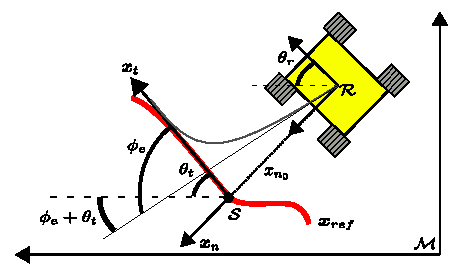
\includegraphics[height=2.5in]{figs/path_follower/orthexp.pdf}
	\caption{Main components of the \ac{ORTHEXP} path following algorithm used in this work.
	In red is the reference trajectory.}
	\label{fig:diff_orthexp}
\end{figure}

In the \ac{GeRoNa} library, commanded longitudinal velocity $v_x$ can be computed based on multiple factors such as upcoming path curvature, current vehicle angular velocity, proximity of obstacles and distance from the end goal.
Due to \ac{ICP} localization noise in the teach phase, the upcoming path curvature would sometimes peak causing the robot to stop on the spot, we therefore removed this factor.
Current vehicle angular velocity has also been removed from the equation to simplify controller parameter tuning.
In our system, no obstacle detection feature is included, meaning that the proximity of obstacles cannot be used as a factor to compute linear velocity.
It is only the distance from the end goal that was used in order to prevent the robot from finishing its course abruptly.
Thus, the commanded linear velocity $v_x$ is computed as
\begin{equation}
\label{eq:exp_lin_vel}
v_x = v_n \exp\left(-\left(\frac{K_g}{d_g}\right)\right),
\end{equation}
where $v_n$ is the target vehicle velocity and $d_g$ is the distance between the robot's pose and the last pose of the final reference trajectory pose. 
At each time step, a new exponential function and command $\bm u$ are computed using the control laws shown in~\autoref{eq:exp_PD} and~\autoref{eq:exp_lin_vel}, using the robot's 2D pose $x_{\text{2D}}$ and reference trajectory $\bm x_{\text{ref}}$ as input.
The parameters for the \ac{ORTHEXP} controller were tuned empirically by having the robot repeating arbitrary short trajectories and minimizing error, these parameters are detailed in~\autoref{tab:orthexp_params}.


\begin{table}[htpb]
	\caption{\ac{ORTHEXP} controller parameters} \label{tab:orthexp_params}
	\begin{center}
		\begin{tabular}{c c | c c | c c}
			% after \\: \hline or \cline{col1-col2} \cline{col3-col4} ...
			General & & Angular velocity & & Linear velocity \\
			\hline
			Waypoint tolerance & \SI{1.0}{m} & $k$ & 0.4 & $K_g$ & 0.5 \\
			Goal tolerance & \SI{0.15}{m} & $K_g$ & 0.5 & $v_n$ & \SI{1.5}{m/s} \\
			 & & $K_h$ & 3.0 & $v_{min}$ & \SI{0.5}{m/s} \\
			 & & Max angular velocity & \SI{1.0}{rad/s} & $v_{max}$ & \SI{1.5}{m/s} \\
		\end{tabular}
	\end{center}
\end{table}

\subsection{Hardware description}
\label{sec:hardware}

Our system was deployed on a Clearpath Robotics Warthog \ac{UGV}, which is shown in~\autoref{fig:warthog}. 
The Warthog is a \ac{SSMR} using two drive units located on each side of its chassis. 
For \acp{SSMR}, steering is done by sending rotating the wheels on each side of the vehicle at different velocities to creating a skidding effect, effectively turning the vehicle.
Vehicle motion control is done through a sub-servo system allowing to control each side's wheel velocity through Sevcon Gen4 drives and aformentionned wheel encoders signal.
A kinematic linear mapping between wheel velocities and body velocities allows to send body-velocity commands directly to the platform.
Finally, the platform is symmetrical, meaning that it is able to drive along each path both forwards and backwards.
The Warthog can be mounted wheels or tracks, for this work, we selected CAMSO ATV T4S tracks in order to maximize mobility. 
The Warthog is also equipped with a differential suspension, maximizing track or wheel traction when navigating steep terrain.
Our vehicle is also equipped with a standard sensor suite for autonomous navigation. 
In order to enable the \ac{LTR} framework, a Robosense RS-32 3D lidar is mounted in front of the robot, for this work, it is the only lidar used for localization.
This lidar has a \SI{200}{m} detection range and produces about \SI{600000}{} points per second.
3 Hall effect sensors are added to each motor to provide wheel odometry for the robot. 
Finally, an XSens MTi-10 \ac{IMU} provides angular velocity and body linear acceleration measurements. 
Additional sensors used for recording in this work include a Dalsa C1920 camera and two Emlid Reach-RS+ \ac {RTK} \ac{GPS} receivers.
Two Robosense RS-16 lidars were added to the rear of the platform to collect measurements on tree canopy but no data was recorded through those sensors. 
All technical specifications for the platform are given in~\autoref{tab:warthog_specs}.


\begin{table}[htpb]
	\caption{Warthog specifications} \label{tab:warthog_specs}
	\begin{center}
		\begin{tabular}{c c | c c}
			\textbf{Physical} &  & \textbf{Power} & \\
			\hline
			% after \\: \hline or \cline{col1-col2} \cline{col3-col4} ...
			Mass & \SI{590}{kg} & Chemistry & AGM sealed lead acid \\ 
			Footprint & 2.13 x 1.52 m & Voltage & \SI{48}{V} \\ 
			Top speed & \SI{18}{km/h} & Capacity & \SI{105}{Ah} \\ 
			Steering geometry & Skid-steering  & Drive & Sevcon Gen4 \\
			Locomotion & CAMSO ATV T4S Tracks \\
			Suspension & Geometric Passive Articulation \\
			\hline
			\textbf{Sensors} & & \textbf{Computing} \\
			\hline
			\ac{LTR} & & Computer & Acrosser AIV-Q170V1FL  \\
			Front lidar & Robosense RS-32 (\SI{10}{Hz}) & CPU & i7-6700 TE \\
			\ac{IMU} & XSens MTi-10 (\SI{100}{Hz}) \\ 
			Wheel encoders & 3 x hall effect sensors (\SI{4}{Hz}) \\
			Recording & &   \\
			Camera & Dalsa C1920 (\SI{8}{Hz})  \\
			\ac{GPS} & Emlid Reach-RS+ (\SI{5}{Hz}) \\
		\end{tabular}
	\end{center}
\end{table}

\begin{SCfigure}
	\centering
	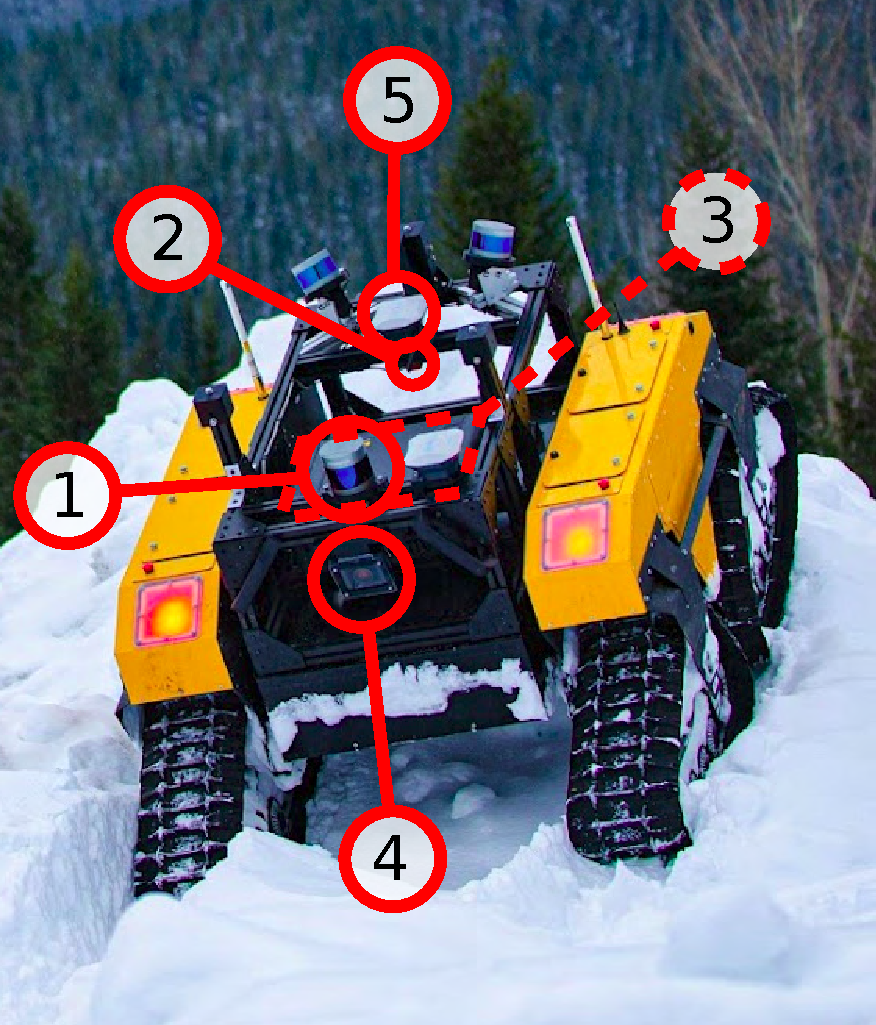
\includegraphics[height=2.5in]{figs/warthog_hardware.pdf}
	\caption{The experimental setup for \ac{LTR} on our Clearpath Robotics Warthog \ac{UGV}: (1) Robosense RS-32 lidar, (2) XSens MTi-10 \ac{IMU}, (3) Acrosser AIV-Q170V1FL computer, (4) Dalsa C1920 color camera, (5) 2 Emlid Reach-RS+ \ac{GPS} antennas.}
	\label{fig:warthog}
\end{SCfigure}
%% To do : Edit Figure to add pointers for all sensors

\section{Environment}
\label{sec:env}

The main focus of this work is deploy our \ac{LTR} framework in a subarctic environment and evaluate it's performance when subject to complex weather conditions.
In order to do so, we conducted our deployments within the \textit{Montmorency} boreal forest, located \SI{70}{km} North of \quebec~city, Canada.
Characteristics of boreal forests include dense closed-crown conifer vegetation~\citep{Russell1988} and long, cold winters leading to a high snow cover on the ground.
Dense vegetation is known to cause an issue for real-time mapping due to static antenna signal being blocked for \ac{RTK} \ac{GNSS}~\citep{Babin2019}.
Snow cover, illumination variation and the uniformity of the environment are also known to be challenging for vision-based approaches~\citep{Paton2017}.
Three different one-way paths were defined, all link 2 \acp{POI}.
The A  and B paths link the Garage and \laverdiere~\acp{POI} through cross-country ski trails, measuring \SI{1.5}{km} and \SI{1.5}{km} respectively.
In order to maximize \ac{UGV} and prevent immobilization, the A and B paths was previously driven on by a snowmobile operator.
The C path connects the Garage and Gazebo \acp{POI} mostly in a larger road network, measuring \SI{0.6}{km}.
The path network is illustrated in~\autoref{fig:forest}.

\begin{figure}[htpb]
	\begin{center}
		\begin{subfigure}[b]{0.45\textwidth}
			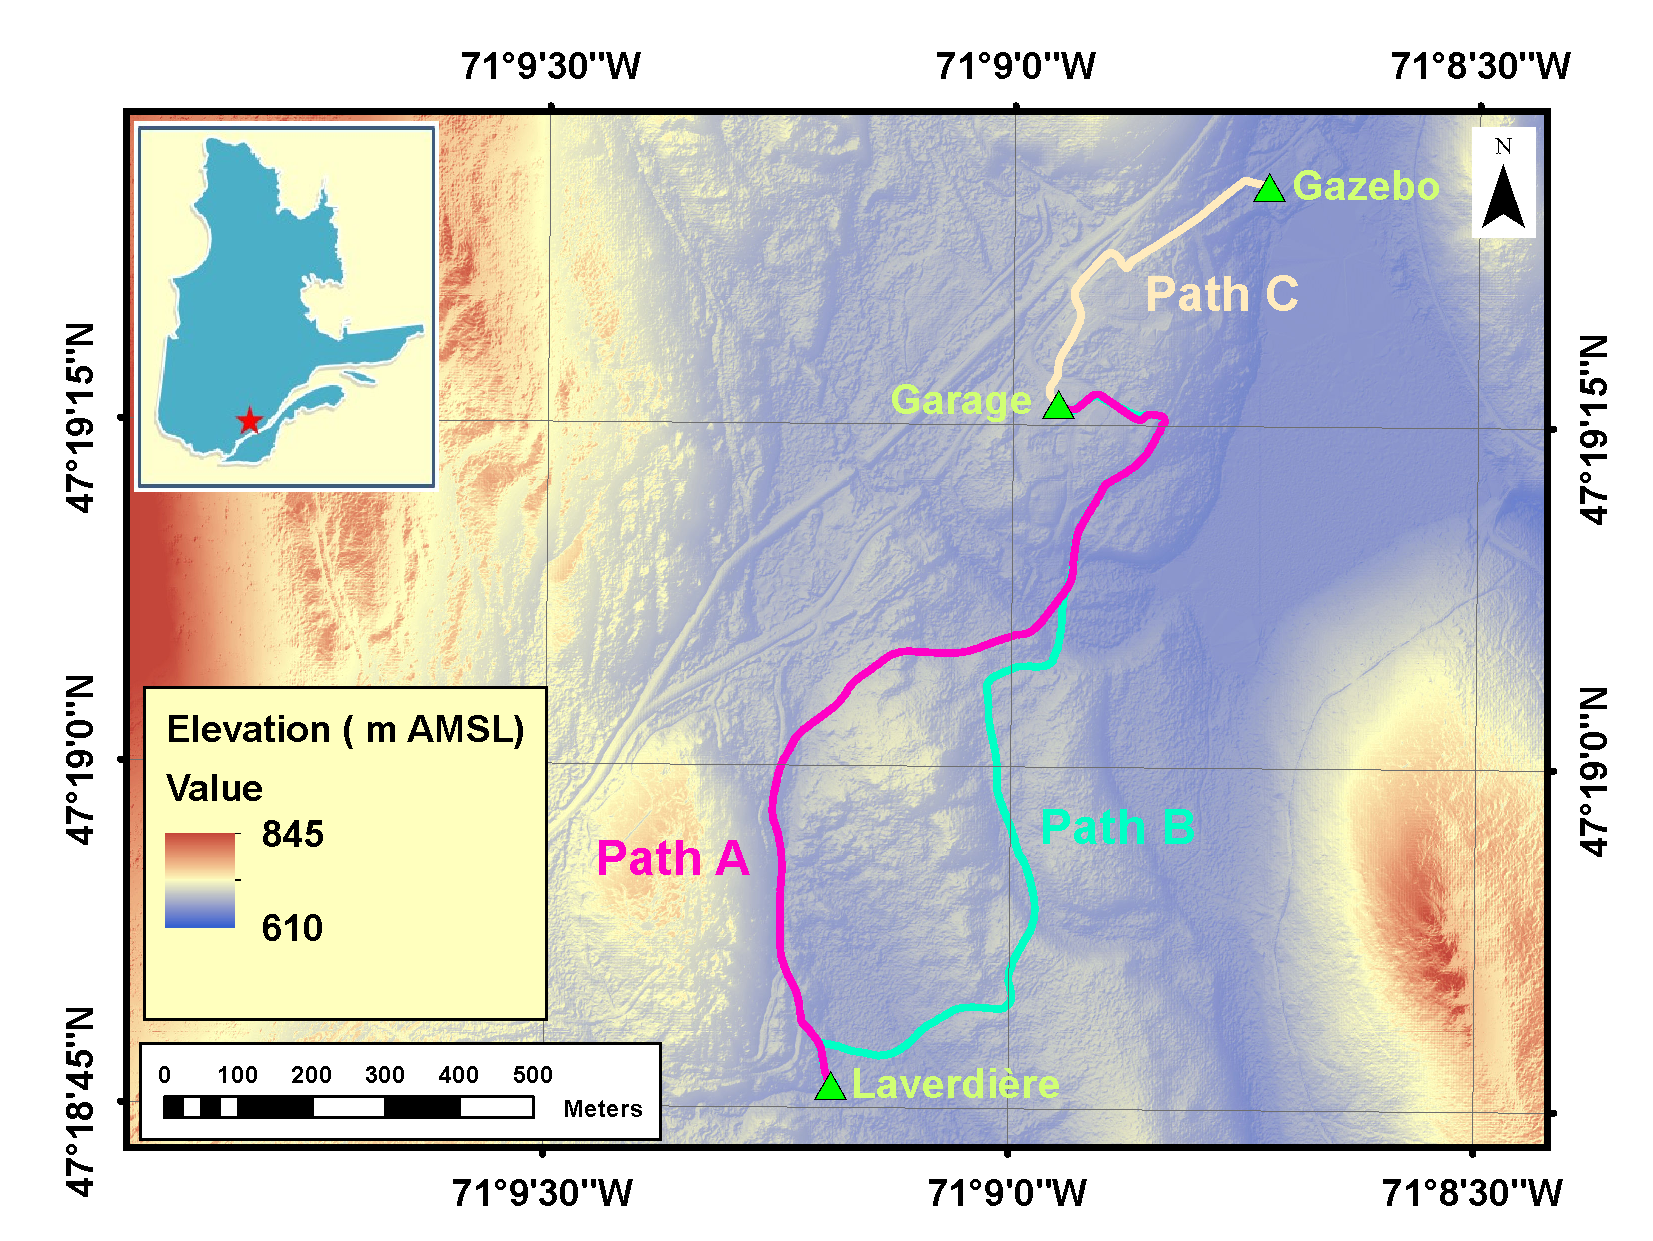
\includegraphics[width=\linewidth]{figs/map-dem.pdf}
			%\caption{A view from above the \textit{Montmorency} forest, which covers \SI{400}{km^2}.}
			\label{fig:view_above}
		\end{subfigure}%
		~~
		\begin{subfigure}[b]{0.45\textwidth}
			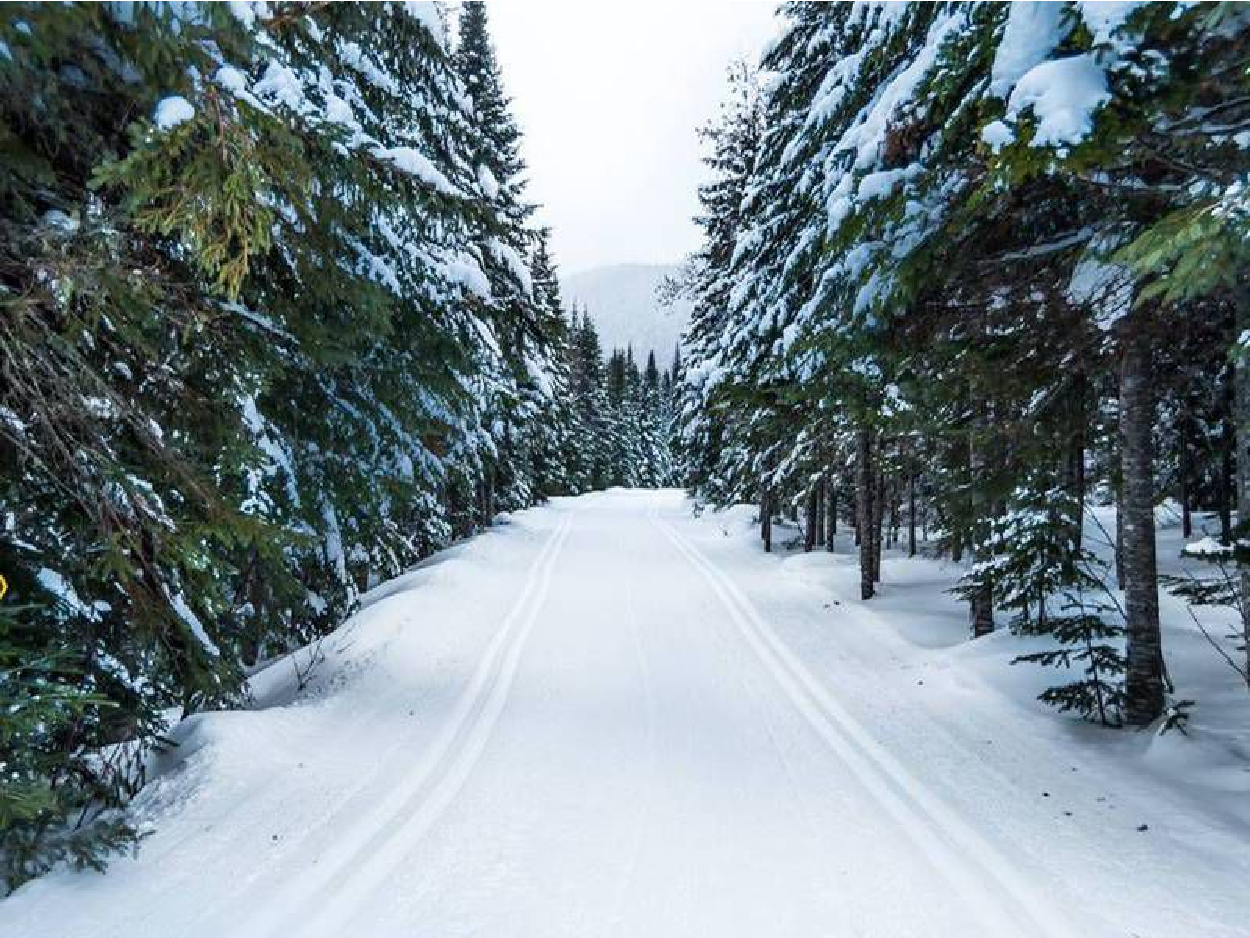
\includegraphics[width=\linewidth]{figs/foret-montmorency-path.pdf}
			%\caption{An example of a snowy path, in which our system performed \ac{LTR}.}
			\label{fig:view_path}
		\end{subfigure}%
		%% Maybe change with a camera image?
		\caption{A digital terrain model of the area where our \ac{LTR} system was deployed.
		We see the three different paths, both the A (\SI{1.5}{km}) and B path ({1.5}{km}) going from the garage \ac{POI} to the \laverdiere~\ac{POI}, while the C path (\SI{0.6}{km}) goes to the Gazebo \ac{POI}.
		The image on the right is an example of the A and B paths, which mostly consists of cross-country sky trails.
		Image credit : \foretmo.} 
		\label{fig:forest}
	\end{center}
\end{figure}

During the five days deployment, we completed
% Discuss weather

\begin{figure} [htpb]
	\centering
	\includegraphics[height=2.0in]{example-image}
	\caption{Johann's various runs and meteo figure}
	\label{fig:meteo_runs}
\end{figure}

\begin{table}[htpb]
	\caption{Overview of all runs realized in this work. 
		All times are defined in the local Eastern Standard Time. 
		The column $\Delta t$ defines the elapsed time since the teach run of the associated path.} \label{tab:all_runs}
	\begin{center}
		\begin{tabular}{c c c c c c}
			\hline
			% after \\: \hline or \cline{col1-col2} \cline{col3-col4} ...
			ID & Path & Start time & Duration & $\Delta t$ & Number of scans \\
			\hline
			TeachA & A & \DTMdate{2021-03-30} \DTMtime{11:04:00} & \DTMtime{00:25:00} & Teach Pass &  \\
			TeachB & B' & \DTMdate{2021-03-29} \DTMtime{15:45:00} & \DTMtime{00:31:00} & Teach Pass \\
			TeachC & C & \DTMdate{2021-03-30} \DTMtime{07:28:00} & \DTMtime{00:15:00} & Teach Pass \\
			R1 & C & \DTMdate{2021-03-31} \DTMtime{10:42:00} & \DTMtime{00:22:00} & \DTMtime{27:14:00} & 17273  \\
			R2 & B & \DTMdate{2021-03-31} \DTMtime{14:03:00} & \DTMtime{00:26:00} & \DTMtime{30:35:00} & 22106  \\
			R3 & A' & \DTMdate{2021-03-31} \DTMtime{15:02:00} & \DTMtime{00:27:00} & \DTMtime{31:34:00} & 16851  \\
			R4 & A & \DTMdate{2021-03-31} \DTMtime{20:42:00} & \DTMtime{00:26:00} & \DTMtime{37:14:00} & 16740  \\
			R5 & B' & \DTMdate{2021-03-31} \DTMtime{21:12:00} & \DTMtime{00:33:00} & \DTMtime{37:44:00} & 18476 \\
			R6 & B & \DTMdate{2021-03-31} \DTMtime{22:00:00} & \DTMtime{00:35:00} & \DTMtime{38:32:00} & 19296 \\
			R7 & A' & \DTMdate{2021-03-31} \DTMtime{22:47:00} & Battery breakdown & \DTMtime{39:19:00} & 10601  \\
			R8 & A & \DTMdate{2021-04-01} \DTMtime{09:21:00} & \DTMtime{00:16:00} & \DTMtime{49:53:00} & 18442  \\
			R9 & B' & \DTMdate{2021-04-01} \DTMtime{10:19:00} & \DTMtime{00:29:00} & \DTMtime{50:51:00} & 20941 \\
			R10 & C & \DTMdate{2021-04-01} \DTMtime{11:01:00} & \DTMtime{00:23:00} & \DTMtime{51:33:00} & 14208 \\
			R11 & B & \DTMdate{2021-04-01} \DTMtime{18:13:00} & \DTMtime{00:23:00} & \DTMtime{58:45:00} & 23214 \\
			R12 & A' & \DTMdate{2021-04-01} \DTMtime{19:09:00} & \DTMtime{00:00:00} & \DTMtime{59:41:00} & 23602 \\
			R13 & A & \DTMdate{2021-04-02} \DTMtime{06:53:00} & \DTMtime{00:26:00} & \DTMtime{71:25:00} & 16840 \\
			R14 & B' & \DTMdate{2021-04-02} \DTMtime{07:25:00} & \DTMtime{00:29:00} & \DTMtime{71:57:00} & 18049 \\
			
		\end{tabular}
	\end{center}
\end{table}

% Check the labels

\begin{figure}[htpb]
	\begin{center}
		\begin{subfigure}[b]{0.32\textwidth}
			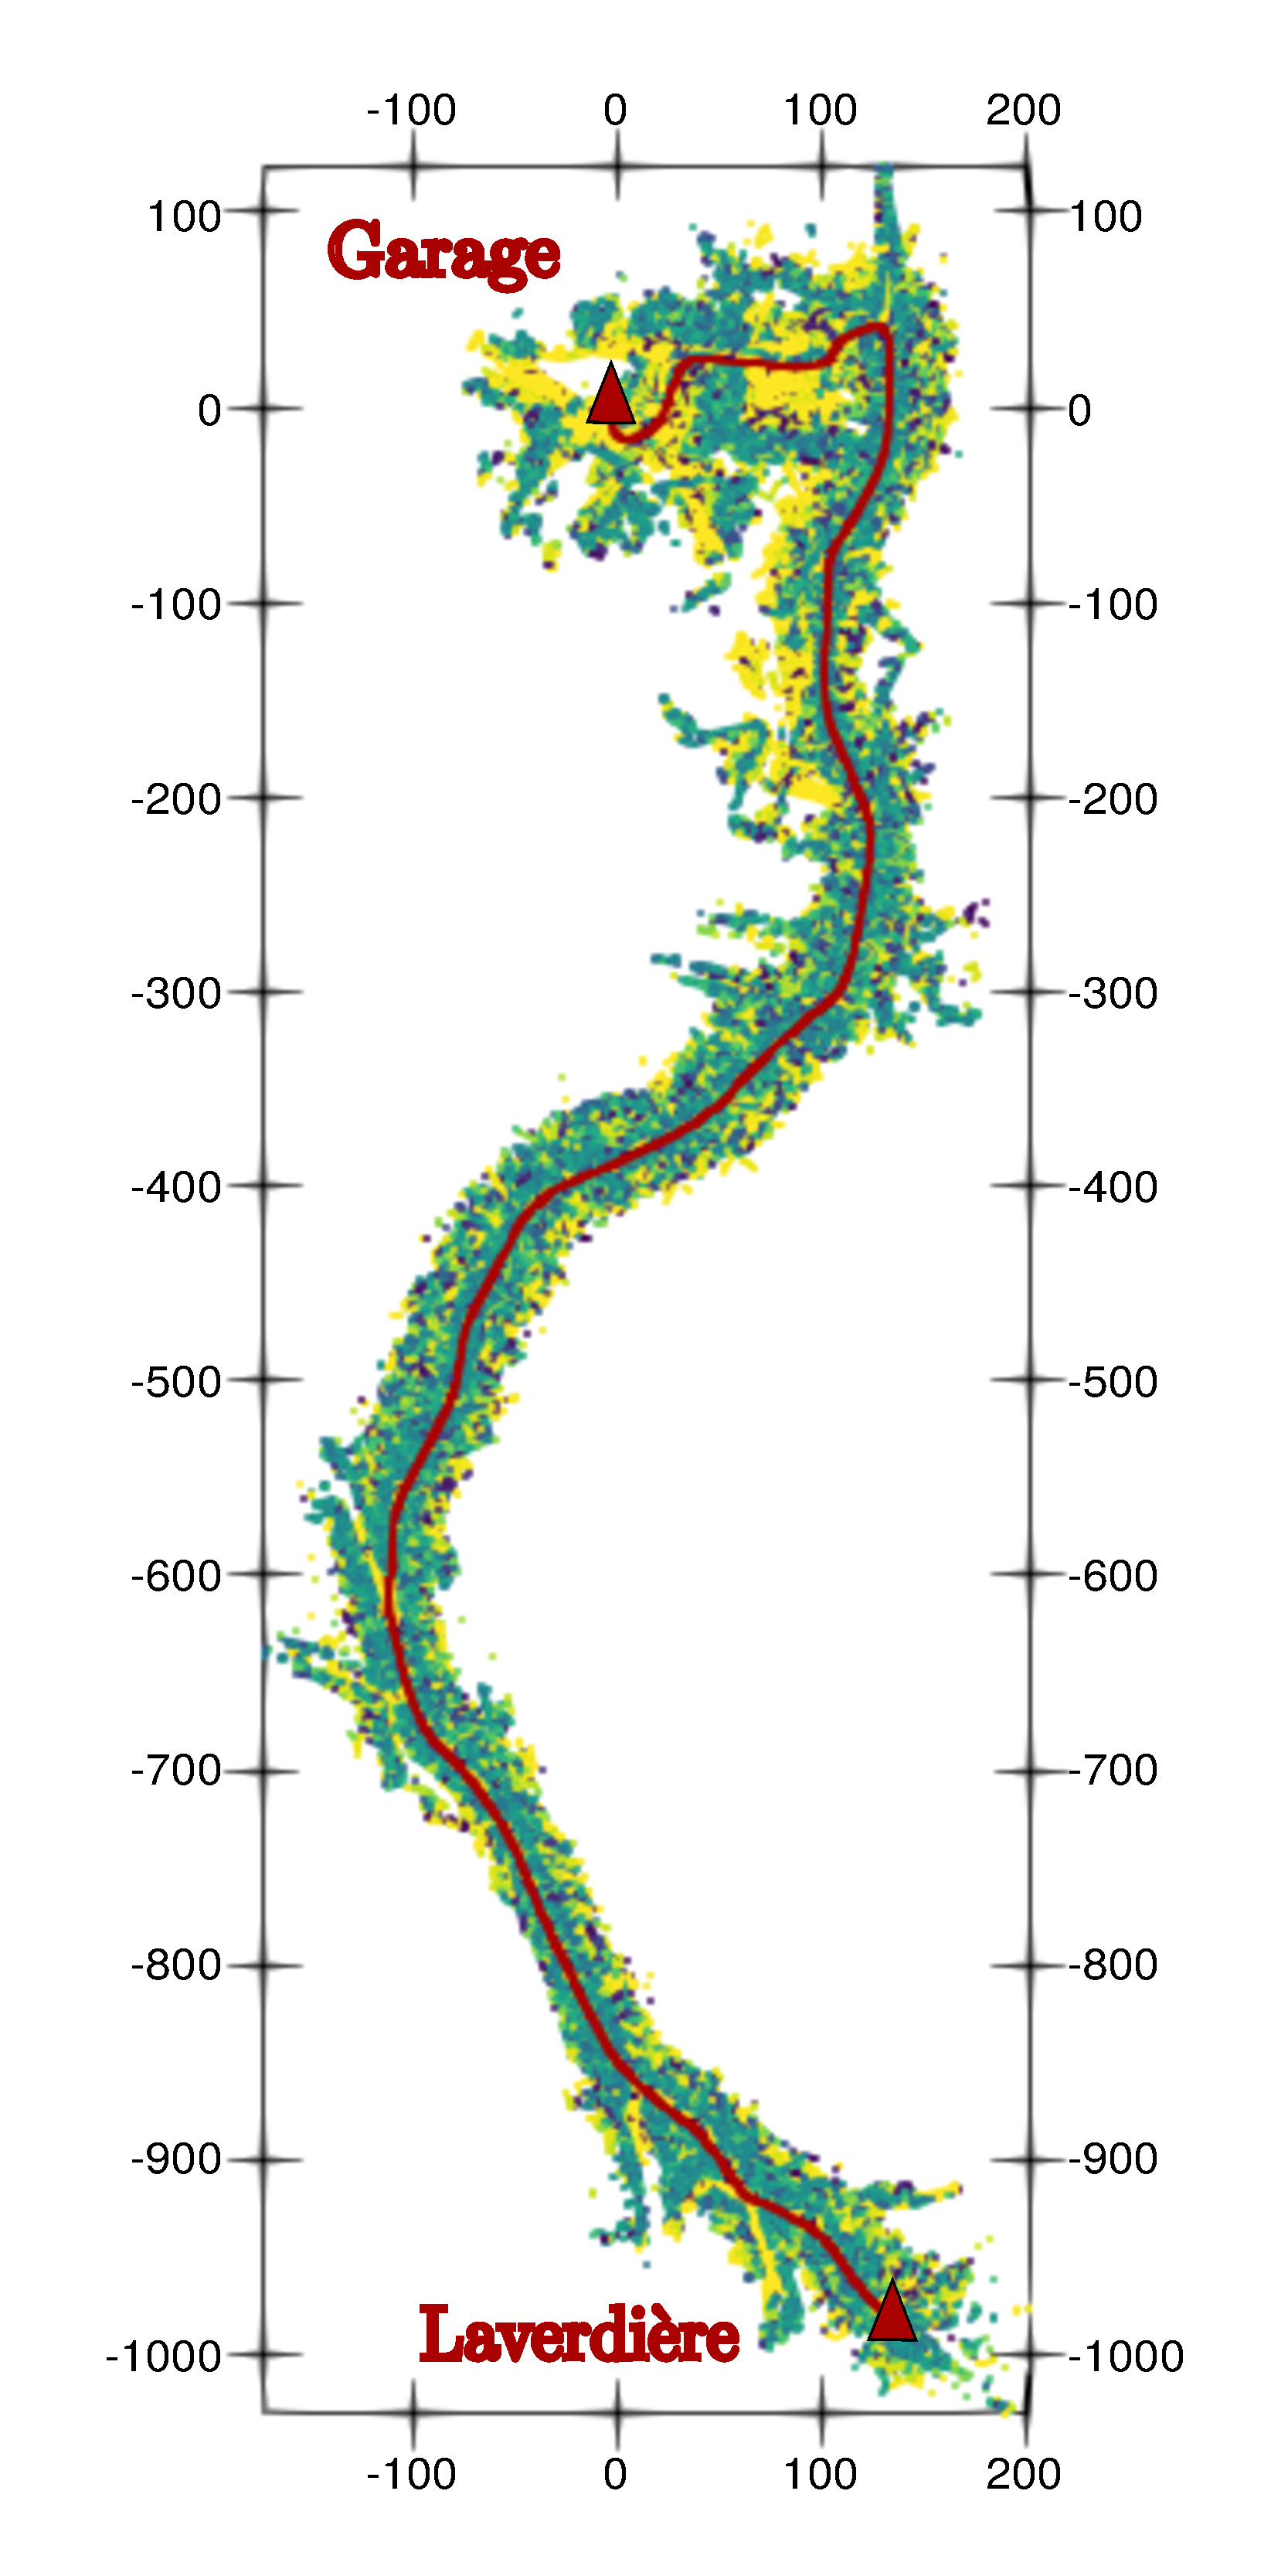
\includegraphics[width=\linewidth]{figs/ltr_map_traj/path_a.pdf}
			%\caption{A view from above the \textit{Montmorency} forest, which covers \SI{400}{km^2}.}
			\label{fig:ltr_a}
			\caption{Path A}
		\end{subfigure}%
		~
		\begin{subfigure}[b]{0.32\textwidth}
			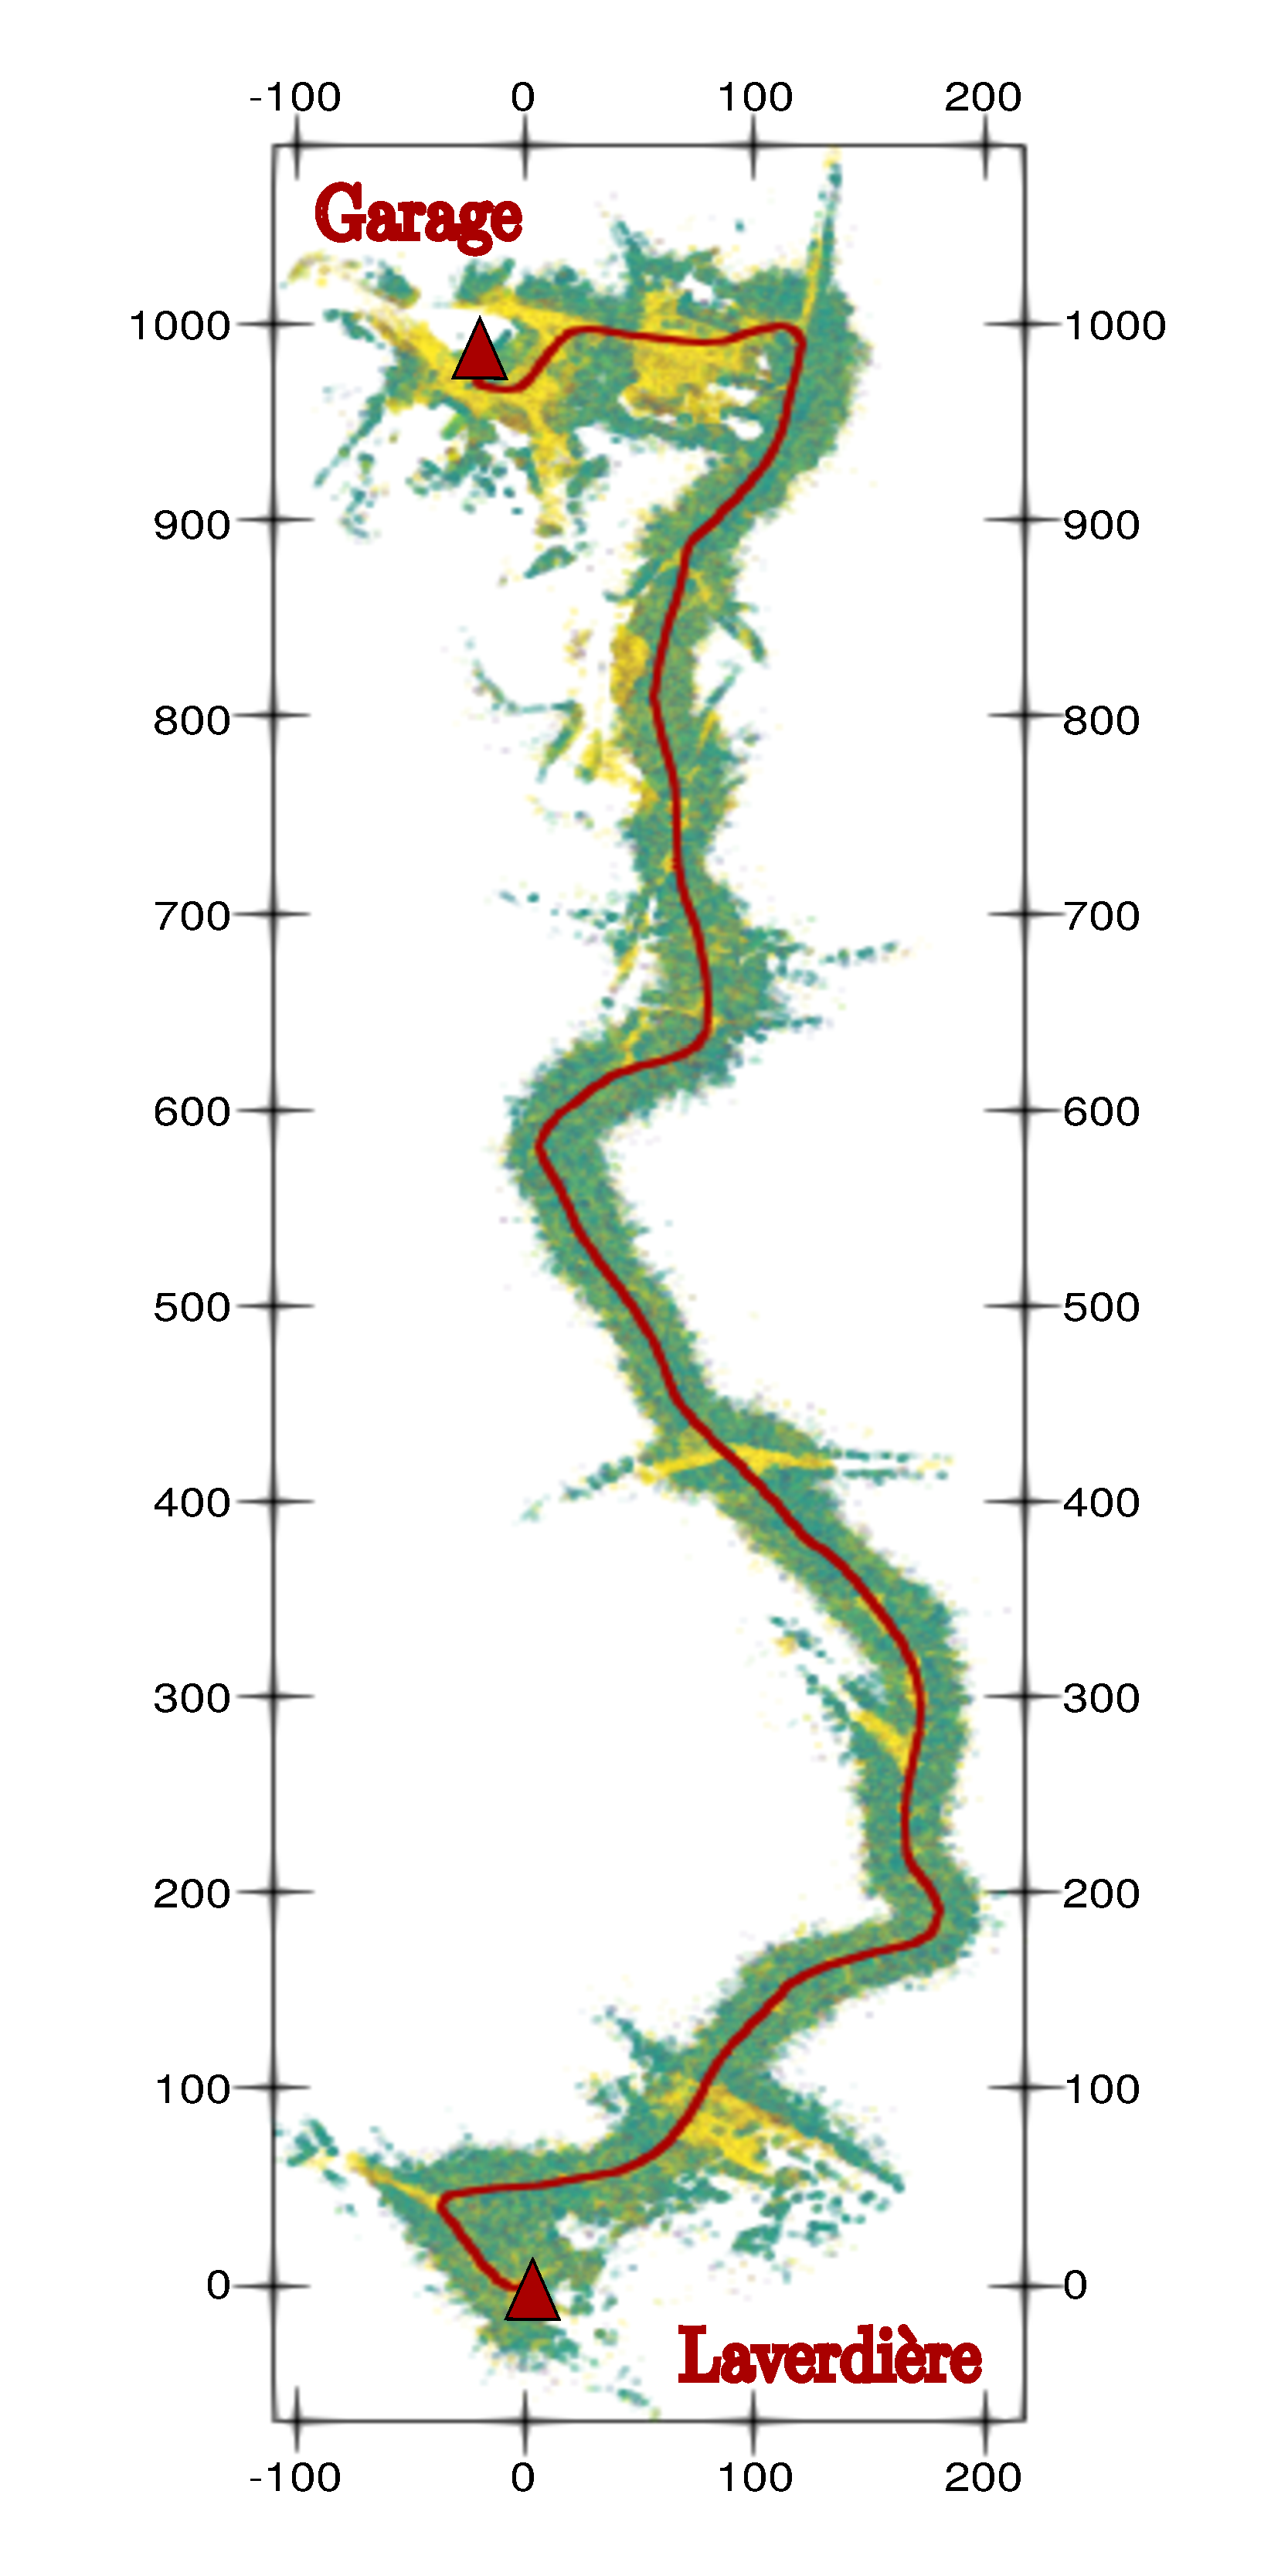
\includegraphics[width=\linewidth]{figs/ltr_map_traj/path_b.pdf}
			%\caption{An example of a snowy path, in which our system performed \ac{LTR}.}
			\label{fig:ltr_b}
			\caption{Path B}
		\end{subfigure}%
		~
		\begin{subfigure}[b]{0.32\textwidth}
			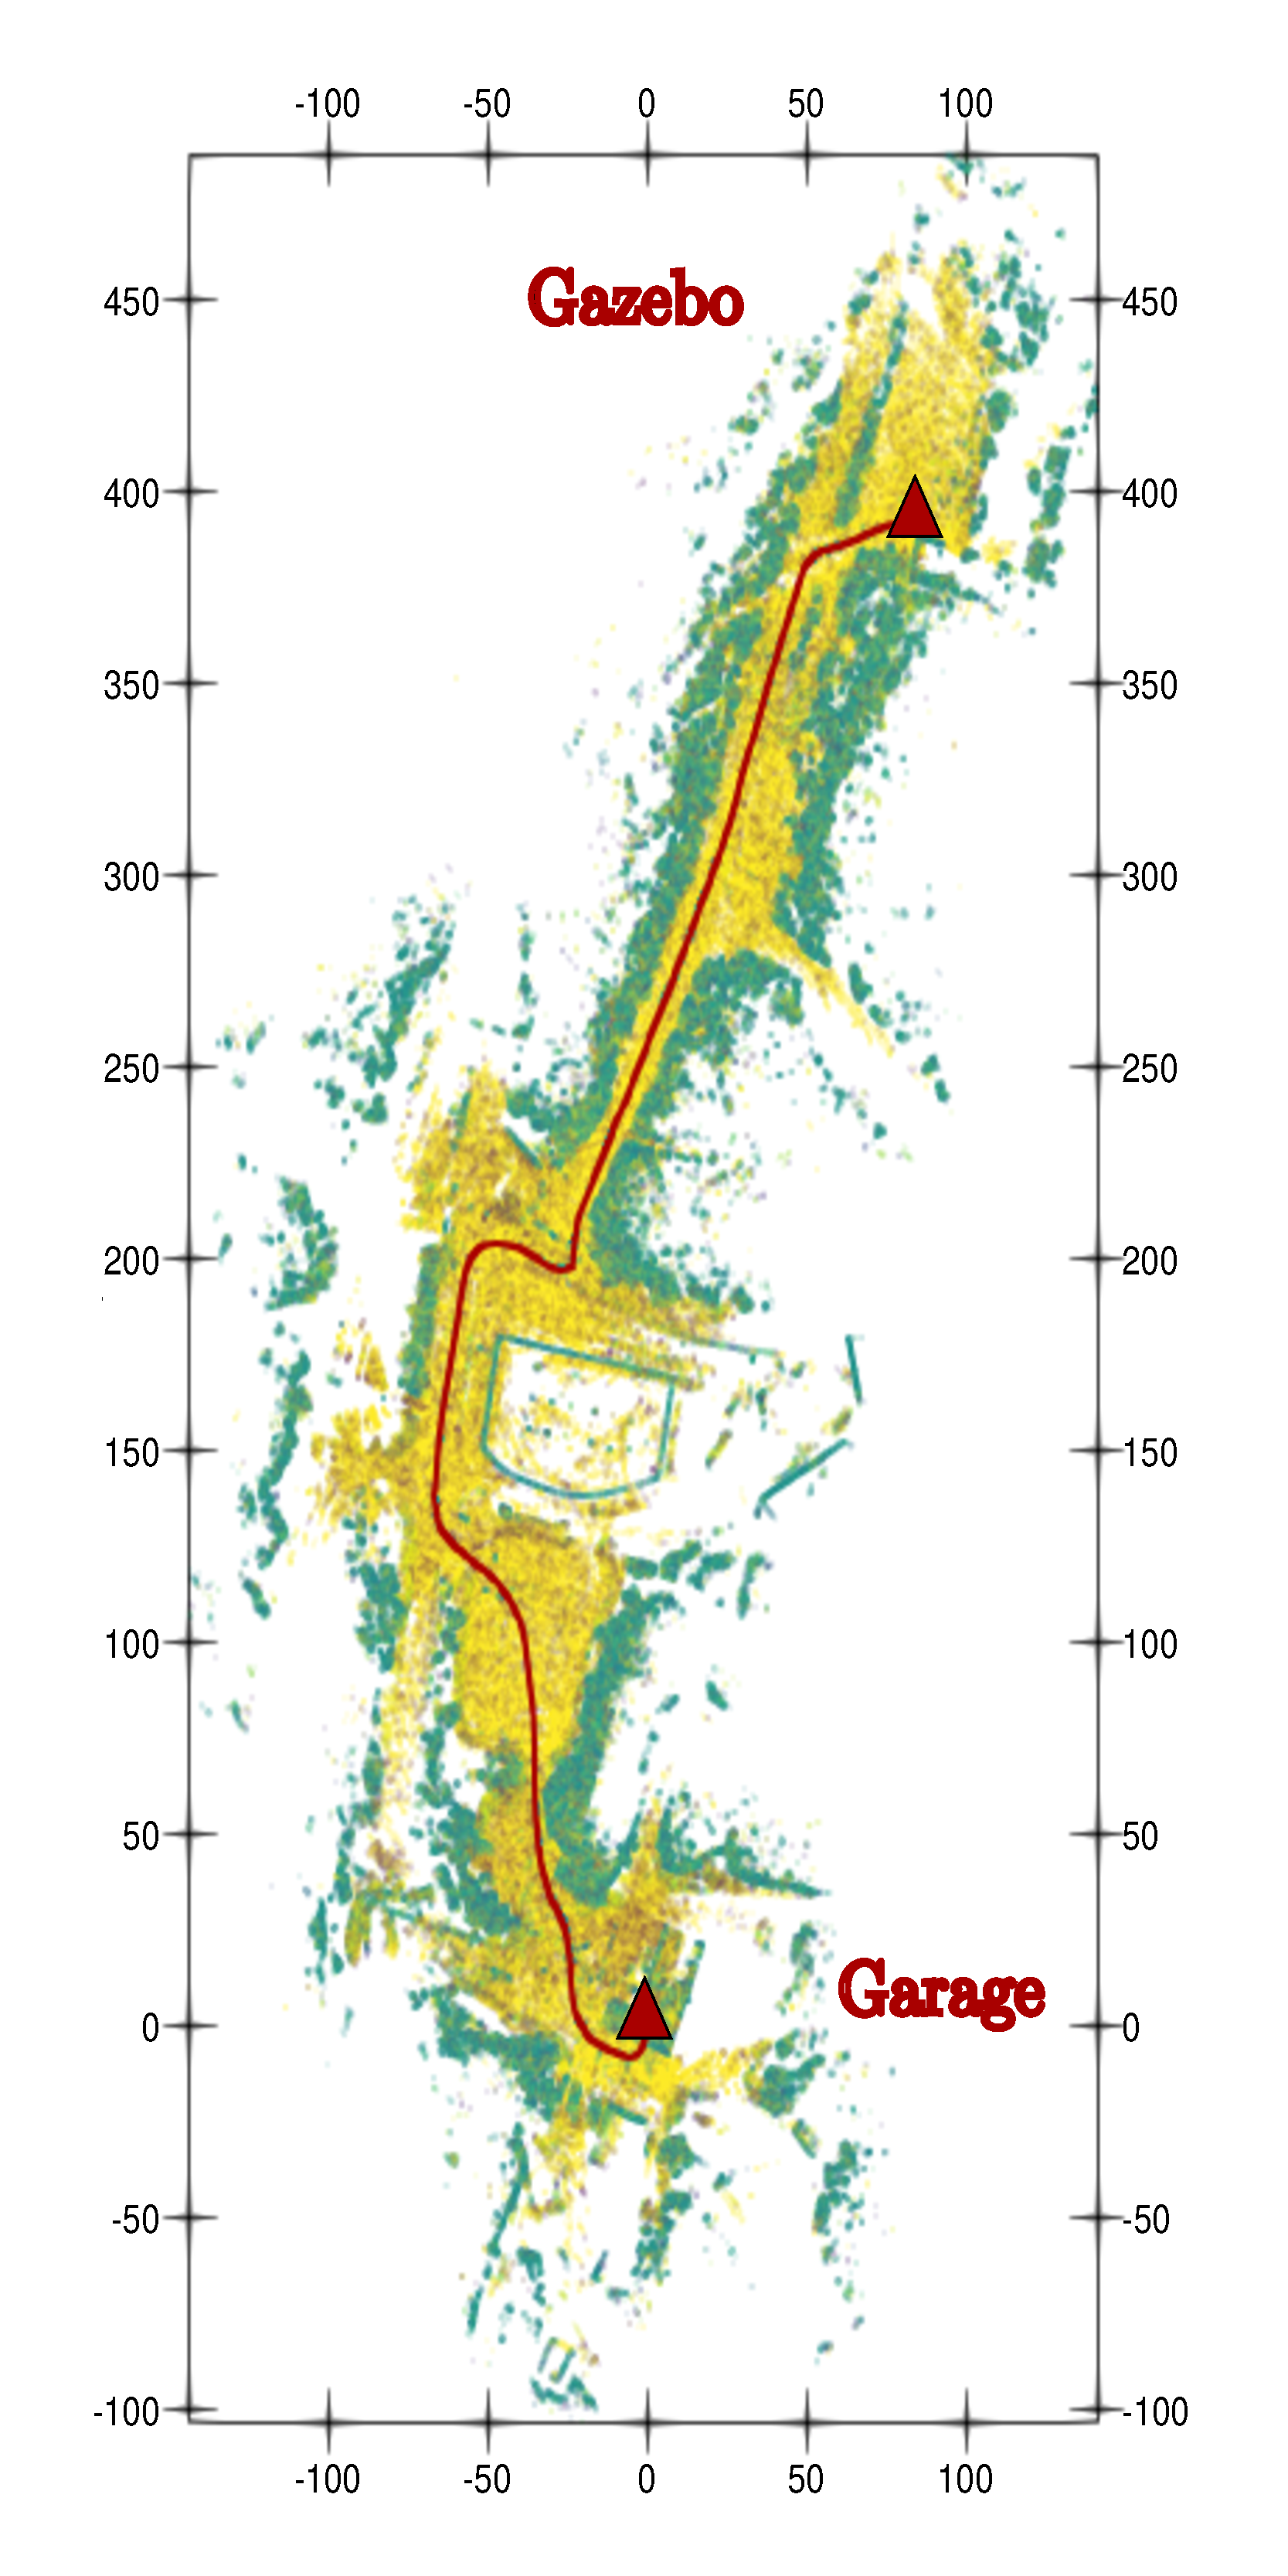
\includegraphics[width=\linewidth]{figs/ltr_map_traj/path_c.pdf}
			%\caption{An example of a snowy path, in which our system performed \ac{LTR}.}
			\label{fig:ltr_c}
			\caption{Path C}
		\end{subfigure}%
		%% Maybe change with a camera image?
		\caption{All reference trajectories and maps recorder for this work.
		In yellow are points with the surface normals pointing upwards, typically representing the ground.
		In green are points with surface normals pointing sideways, typically representing walls or trees.
		In red is the reference trajectory and their respective \acp{POI}.} 
		\label{fig:forest}
	\end{center}
\end{figure}

% Validate run durations through bag files

% Number of points per maps : 
%Map A: 1729505 points
%Map B: 2423769 points
%Map C: 637690 points

\lightlipsum[1]
\section{Results}
\label{sec:results}

\lightlipsum[1]

\begin{figure} [htpb]
	\centering
	\includegraphics[height=2.0in]{example-image}
	\caption{Reference maps and trajectories for all paths}
	\label{fig:ref_paths}
\end{figure}


\subsection{Localization}
\label{sec:res_loc}

\lightlipsum[1]

\subsubsection{Vision-based}
\label{sec:res_vis}

\lightlipsum[1]

\begin{figure} [htpb]
	\centering
	\includegraphics[height=2.0in]{example-image}
	\caption{Olivier's over and under exposition figure for cameras}
	\label{fig:cameras_expo}
\end{figure}

\subsubsection{GNSS}
\label{sec:res_gnss}

\lightlipsum[1]

\begin{figure} [htpb]
	\centering
	\includegraphics[height=2.0in]{example-image}
	\caption{Maxime's GNSS error figure}
	\label{fig:gnss_error}
\end{figure}

\subsubsection{ICP}
\label{sec:ICP}

\lightlipsum[1]

\begin{figure} [htpb]
	\centering
	\includegraphics[height=2.0in]{example-image}
	\caption{Figure explaining ICP error for every run (correlated with meteo).}
	\label{fig:icp_error}
\end{figure}

\begin{figure} [htpb]
	\centering
	\includegraphics[height=2.0in]{example-image}
	\caption{Figure explaining special cases when mapping needed to be enabled.}
	\label{fig:icp_failure}
\end{figure}

\subsection{Motion and control}
\label{sec:res_motion}

\lightlipsum[1]

\subsubsection{Path following error}
\label{sec:cmd_error}

\lightlipsum[1]

\begin{figure} [htpb]
	\centering
	\includegraphics[height=2.0in]{example-image}
	\caption{Dominic's path following error figure}
	\label{fig:pf_error}
\end{figure}

\subsubsection{Command error and power consumption}
\label{sec:cmd_error}

\lightlipsum[1]

\begin{figure} [htpb]
	\centering
	\includegraphics[height=2.0in]{example-image}
	\caption{Power consumption / motion efficiency figure.}
	\label{fig:moiton_power}
\end{figure}
\section{Lessons learned}
\label{sec:lessons}

\lightlipsum[1]
\lightlipsum[1]
\section{Conclusion}
\label{sec:concl}

\lightlipsum[1]

\subsubsection*{Acknowledgments}
This research was supported by the Natural Sciences and Engineering Research Council of Canada (NSERC) through the grant CRDPJ 527642-18 SNOW (Self-driving Navigation Optimized for Winter) and FORAC.

% To add : Damien's dad, meteorological lab



%\bibliographystyle{apalike}
%\bibliography{references.bib}
\printbibliography


\end{document}



